\documentclass[12pt]{article}

\usepackage{tikz}

\begin{document}
	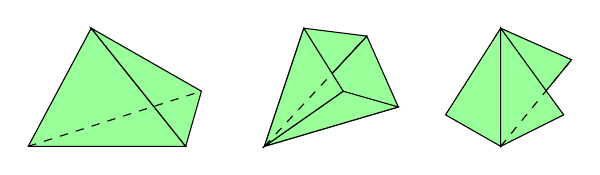
\begin{tikzpicture}
		% We need to define the drawing style
		[edges/.style={black, dashed},
		faces/.style={fill=green!40!white, draw=black}]
	
		% First a tetrahedron
		\begin{scope}[xshift=0cm]
			\coordinate (A) at (0,0);
			\coordinate (B) at (2,0);
			\coordinate (C) at (0.8,1.5);
			\coordinate (D) at (2.2,0.7);
			
			\filldraw[faces] (A) -- (B) -- (C) -- cycle;
			\filldraw[faces] (B) -- (C) -- (D) -- cycle;
			\draw[edges] (A) -- (D);
		\end{scope}
		
		% Second: four triangles in the form of a cone
		\begin{scope}[xshift=3cm]
			\coordinate (A) at (0,0);
			\coordinate (B) at (1.7,0.5);
			\coordinate (C) at (1.3,1.4);
			\coordinate (D) at (0.5,1.5);
			\coordinate (E) at (1,0.7);
			
			% Take care to draw the faces in the back first
			\filldraw[faces] (A) -- (B) -- (C) -- cycle;
			\filldraw[faces] (A) -- (C) -- (D) -- cycle;
			% Now the faces in the front
			\filldraw[faces] (A) -- (B) -- (E) -- cycle;
			\filldraw[faces] (A) -- (E) -- (D) -- cycle;
			% Finally the dashed line for the "hidden" edge
			\draw[edges] (A) -- (C);
		\end{scope}
		
		% Three triangles that share an edge
		\begin{scope}[xshift=6cm]
			\coordinate (A) at (0,0);
			\coordinate (B) at (0,1.5);
			\coordinate (C) at (-0.7,0.4);
			\coordinate (D) at (0.8,0.4);
			\coordinate (E) at (0.9,1.1);
			
			% draw back face first
			\filldraw[faces] (A) -- (B) -- (E) -- cycle;
			% Now draw front faces
			\filldraw[faces] (A) -- (B) -- (C) -- cycle;
			\filldraw[faces] (A) -- (B) -- (D) -- cycle;
			% Draw dashed line
			\draw[edges] (A) -- (E);
		\end{scope}
	\end{tikzpicture}
\end{document}